%Draw pipeline%
\subsection{Bài toán}
\subsubsection{Pedestrian Detection (Nhận diện người đi bộ)}
Bài toán nhận diện người đi bộ là một bài toán trong lĩnh vực thị giác máy tính, có mục tiêu nhằm xác định và định vị vị trí của người đi bộ trong các hình ảnh hoặc video. Trong đề tài này, nhóm chỉ có khả năng nhận diện người đi bộ trong các hình ảnh. Mục tiêu của bài toán là xác định và định vị người đi bộ trong hình ảnh, cung cấp thông tin về vị trí, bounding box và lớp (như người đi bộ hay không).

Input: Một hình ảnh kỹ thuật số (hay single frame)

Output: Một hình ảnh bao gồm các tọa độ (bounding boxes) biểu thị cho vị trí của người đi bộ trong hình (nếu có).
\vfill
\graphicspath{{figures/}}
\begin{figure}[h!]
    \centering
    \subfloat[\centering Input]{{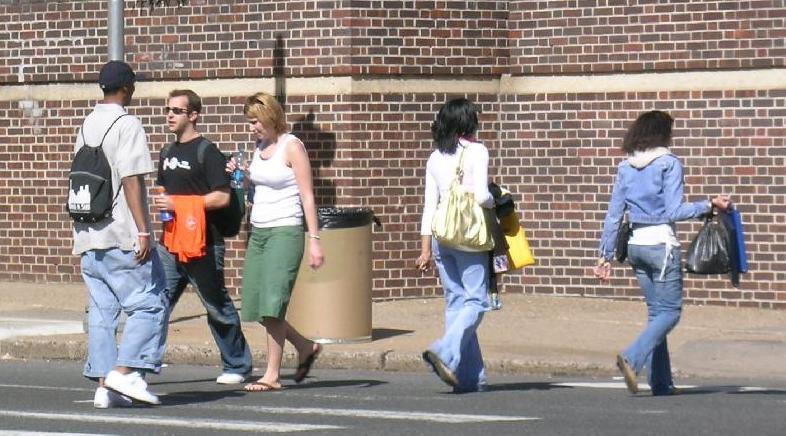
\includegraphics[width=7cm]{graphics/image_11.jpg} }}
    \qquad
    \subfloat[\centering Output]{{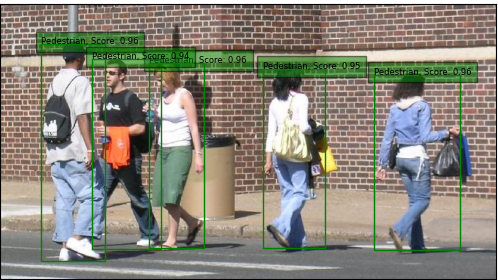
\includegraphics[width=7cm]{graphics/predicted_11.png} }}
    \caption{Một ví dụ về input và output của bài toán}
\end{figure}
\subsection{Pipeline}
Các kỹ thuật Object Detection truyền thống thường tuân theo ba bước chính được đưa ra trong hình bên dưới.

Bước đầu tiên liên quan đến việc tạo ra một số vùng đề xuất (region proposal). Từ mỗi vùng đề xuất, một vectơ đặc trưng có độ dài cố định được trích xuất bằng cách sử dụng các image descriptors khác nhau ví dụ như histogram of oriented gradients (HOG). Vector đặc trưng sau đó được sử dụng để phân loại mỗi vùng đề xuất vào lớp nền hoặc vào một trong các lớp đối tượng cụ thể. Khi số lượng lớp tăng lên, độ phức tạp của việc xây dựng một mô hình có thể phân biệt được tất cả các đối tượng này cũng tăng lên. Một trong những mô hình phổ biến được sử dụng để phân loại các vùng đề xuất là support vector machine (SVM).
\graphicspath{{figures/}}
\begin{figure}[h!]
  \centering
  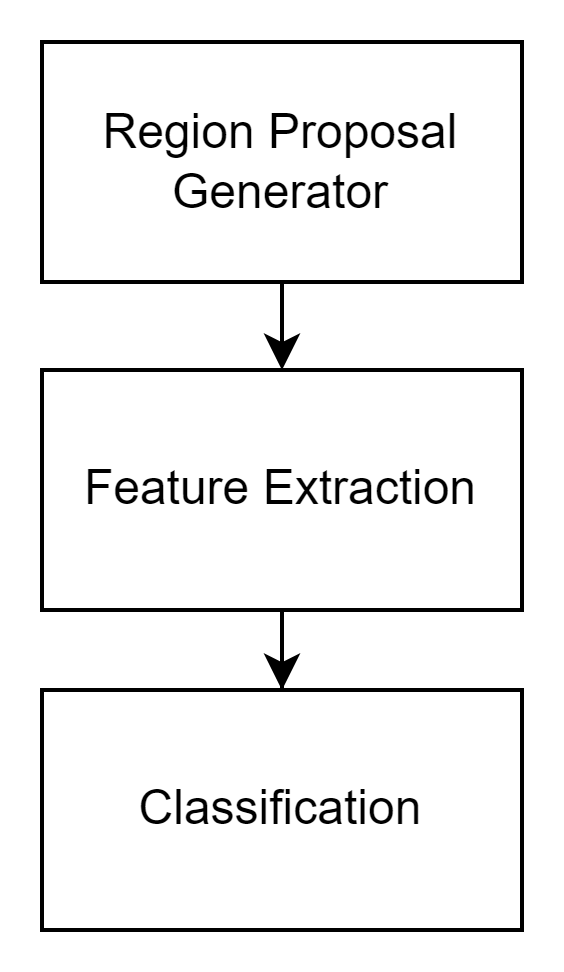
\includegraphics[scale=0.25]{graphics/pipeline.png}
  \caption{Pipeline của các phương pháp truyền thống trong Object Detection}
\end{figure}
